\documentclass[a4paper,12pt]{report}

%%% HarrixLaTeXDocumentTemplate
%%% Версия 1.22
%%% Шаблон документов в LaTeX на русском языке. Данный шаблон применяется в проектах HarrixTestFunctions, MathHarrixLibrary, Standard-Genetic-Algorithm  и др.
%%% https://github.com/Harrix/HarrixLaTeXDocumentTemplate
%%% Шаблон распространяется по лицензии Apache License, Version 2.0.

%%% Проверка используемого TeX-движка %%%
\usepackage{ifxetex}

%%% Поля и разметка страницы %%%
\usepackage{lscape} % Для включения альбомных страниц
\usepackage{geometry} % Для последующего задания полей

%%% Кодировки и шрифты %%%
\ifxetex
\usepackage{polyglossia} % Поддержка многоязычности
\usepackage{fontspec} % TrueType-шрифты
\else
\usepackage{cmap}  % Улучшенный поиск русских слов в полученном pdf-файле
\usepackage[T2A]{fontenc} % Поддержка русских букв
\usepackage[utf8]{inputenc} % Кодировка utf8
\usepackage[english, russian]{babel} % Языки: русский, английский
\usepackage{ textcomp }

\IfFileExists{pscyr.sty}{\usepackage{pscyr}}{} % Красивые русские шрифты
\fi

%%% Математические пакеты %%%
\usepackage{amsthm,amsfonts,amsmath,amssymb,amscd} % Математические дополнения от AMS
% Для жиного курсива в формулах %
\usepackage{bm}
% Для рисования некоторых математических символов (например, закрашенных треугольников)
\usepackage{mathabx}

%%% Оформление абзацев %%%
\usepackage{indentfirst} % Красная строка
\usepackage{setspace} % Расстояние между строками
\usepackage{enumitem} % Для список обнуление расстояния до абзаца

%%% Цвета %%%
\usepackage[usenames]{color}
\usepackage{color}
\usepackage{colortbl}

%%% Таблицы %%%
\usepackage{longtable} % Длинные таблицы
\usepackage{multirow,makecell,array} % Улучшенное форматирование таблиц

%%% Общее форматирование
\usepackage[singlelinecheck=off,center]{caption} % Многострочные подписи
\usepackage{soul} % Поддержка переносоустойчивых подчёркиваний и зачёркиваний
\usepackage{icomma} % Запятая в десятичных дробях

%%% Библиография %%%
\usepackage{cite}

%%% Гиперссылки %%%
\usepackage{hyperref}

%%% Изображения %%%
\usepackage{graphicx} % Подключаем пакет работы с графикой
\usepackage{epstopdf}
\usepackage{subcaption}

%%% Оглавление %%%
\usepackage{tocloft}

%%% Колонтитулы %%%
\usepackage{fancyhdr}

%%% Отображение кода %%%
\usepackage{xcolor}
\usepackage{listings}
\usepackage{caption}

%%% Псевдокоды %%%
\usepackage{algorithm} 
\usepackage{algpseudocode}

%%% Рисование графиков %%%
\usepackage{pgfplots}

%%% Обтекание рисунка %%%
\usepackage{wrapfig}
 %Подключаем модуль пакетов
%%% HarrixLaTeXDocumentTemplate
%%% Версия 1.22
%%% Шаблон документов в LaTeX на русском языке. Данный шаблон применяется в проектах HarrixTestFunctions, MathHarrixLibrary, Standard-Genetic-Algorithm  и др.
%%% https://github.com/Harrix/HarrixLaTeXDocumentTemplate
%%% Шаблон распространяется по лицензии Apache License, Version 2.0.

%%% Макет страницы %%%
% Выставляем значения полей (ГОСТ 7.0.11-2011, 5.3.7)
\geometry{a4paper,top=2cm,bottom=2cm,left=2.5cm,right=1cm}

%%% Выравнивание и переносы %%%
\sloppy % Избавляемся от переполнений
\clubpenalty=10000 % Запрещаем разрыв страницы после первой строки абзаца
\widowpenalty=10000 % Запрещаем разрыв страницы после последней строки абзаца


%%% Библиография %%%
\makeatletter
\bibliographystyle{utf8gost71u}  % Оформляем библиографию по ГОСТ 7.1 (ГОСТ Р 7.0.11-2011, 5.6.7)
\renewcommand{\@biblabel}[1]{#1.} % Заменяем библиографию с квадратных скобок на точку
\makeatother

%%% Изображения %%%
\graphicspath{{images/}} % Пути к изображениям
% Поменять двоеточние на точку в подписях к рисунку
\RequirePackage{caption}
\DeclareCaptionLabelSeparator{defffis}{. }
\captionsetup{justification=centering,labelsep=defffis}

%%% Абзацы %%%
% Отсупы между строками
\singlespacing
\setlength{\parskip}{0.3cm} % отступы между абзацами
\linespread{1.3} % Полуторный интвервал (ГОСТ Р 7.0.11-2011, 5.3.6)

% Оформление списков
\setlist{leftmargin=1.5cm,topsep=0pt}
% Используем дефис для ненумерованных списков (ГОСТ 2.105-95, 4.1.7)
\renewcommand{\labelitemi}{\normalfont\bfseries{--}}

%%% Цвета %%%
% Цвета для кода
\definecolor{string}{HTML}{B40000} % цвет строк в коде
\definecolor{comment}{HTML}{008000} % цвет комментариев в коде
\definecolor{keyword}{HTML}{1A00FF} % цвет ключевых слов в коде
\definecolor{morecomment}{HTML}{8000FF} % цвет include и других элементов в коде
\definecolor{сaptiontext}{HTML}{FFFFFF} % цвет текста заголовка в коде
\definecolor{сaptionbk}{HTML}{999999} % цвет фона заголовка в коде
\definecolor{bk}{HTML}{FFFFFF} % цвет фона в коде
\definecolor{frame}{HTML}{999999} % цвет рамки в коде
\definecolor{brackets}{HTML}{B40000} % цвет скобок в коде
% Цвета для гиперссылок
\definecolor{linkcolor}{HTML}{799B03} % цвет ссылок
\definecolor{urlcolor}{HTML}{799B03} % цвет гиперссылок
\definecolor{citecolor}{HTML}{799B03} % цвет гиперссылок
\definecolor{gray}{rgb}{0.4,0.4,0.4}
\definecolor{tableheadcolor}{HTML}{E5E5E5} % цвет шапки в таблицах
\definecolor{darkblue}{rgb}{0.0,0.0,0.6}
% Цвета для графиков
\definecolor{plotcoordinate}{HTML}{88969C}% цвет точек на координатых осях (минимум и максимум)
\definecolor{plotgrid}{HTML}{ECECEC} % цвет сетки
\definecolor{plotmain}{HTML}{97BBCD} % цвет основного графика
\definecolor{plotsecond}{HTML}{FF0000} % цвет второго графика, если графика только два
\definecolor{plotsecondgray}{HTML}{CCCCCC} % цвет второго графика, если графика только два. В сером виде.
\definecolor{darkgreen}{HTML}{799B03} % цвет темно-зеленого

%%% Отображение кода %%%
% Настройки отображения кода
\lstset{
language=C++, % Язык кода по умолчанию
morekeywords={*,...}, % если хотите добавить ключевые слова, то добавляйте
% Цвета
keywordstyle=\color{keyword}\ttfamily\bfseries,
%stringstyle=\color{string}\ttfamily,
stringstyle=\ttfamily\color{red!50!brown},
commentstyle=\color{comment}\ttfamily\itshape,
morecomment=[l][\color{morecomment}]{\#}, 
% Настройки отображения     
breaklines=true, % Перенос длинных строк
basicstyle=\ttfamily\footnotesize, % Шрифт для отображения кода
backgroundcolor=\color{bk}, % Цвет фона кода
frame=lrb,xleftmargin=\fboxsep,xrightmargin=-\fboxsep, % Рамка, подогнанная к заголовку
rulecolor=\color{frame}, % Цвет рамки
tabsize=3, % Размер табуляции в пробелах
% Настройка отображения номеров строк. Если не нужно, то удалите весь блок
%numbers=left, % Слева отображаются номера строк
%stepnumber=1, % Каждую строку нумеровать
%numbersep=5pt, % Отступ от кода 
%numberstyle=\small\color{black}, % Стиль написания номеров строк
% Для отображения русского языка
extendedchars=true,
literate={Ö}{{\"O}}1
  {Ä}{{\"A}}1
  {Ü}{{\"U}}1
  {ß}{{\ss}}1
  {ü}{{\"u}}1
  {ä}{{\"a}}1
  {ö}{{\"o}}1
  {~}{{\textasciitilde}}1
  {а}{{\selectfont\char224}}1
  {б}{{\selectfont\char225}}1
  {в}{{\selectfont\char226}}1
  {г}{{\selectfont\char227}}1
  {д}{{\selectfont\char228}}1
  {е}{{\selectfont\char229}}1
  {ё}{{\"e}}1
  {ж}{{\selectfont\char230}}1
  {з}{{\selectfont\char231}}1
  {и}{{\selectfont\char232}}1
  {й}{{\selectfont\char233}}1
  {к}{{\selectfont\char234}}1
  {л}{{\selectfont\char235}}1
  {м}{{\selectfont\char236}}1
  {н}{{\selectfont\char237}}1
  {о}{{\selectfont\char238}}1
  {п}{{\selectfont\char239}}1
  {р}{{\selectfont\char240}}1
  {с}{{\selectfont\char241}}1
  {т}{{\selectfont\char242}}1
  {у}{{\selectfont\char243}}1
  {ф}{{\selectfont\char244}}1
  {х}{{\selectfont\char245}}1
  {ц}{{\selectfont\char246}}1
  {ч}{{\selectfont\char247}}1
  {ш}{{\selectfont\char248}}1
  {щ}{{\selectfont\char249}}1
  {ъ}{{\selectfont\char250}}1
  {ы}{{\selectfont\char251}}1
  {ь}{{\selectfont\char252}}1
  {э}{{\selectfont\char253}}1
  {ю}{{\selectfont\char254}}1
  {я}{{\selectfont\char255}}1
  {А}{{\selectfont\char192}}1
  {Б}{{\selectfont\char193}}1
  {В}{{\selectfont\char194}}1
  {Г}{{\selectfont\char195}}1
  {Д}{{\selectfont\char196}}1
  {Е}{{\selectfont\char197}}1
  {Ё}{{\"E}}1
  {Ж}{{\selectfont\char198}}1
  {З}{{\selectfont\char199}}1
  {И}{{\selectfont\char200}}1
  {Й}{{\selectfont\char201}}1
  {К}{{\selectfont\char202}}1
  {Л}{{\selectfont\char203}}1
  {М}{{\selectfont\char204}}1
  {Н}{{\selectfont\char205}}1
  {О}{{\selectfont\char206}}1
  {П}{{\selectfont\char207}}1
  {Р}{{\selectfont\char208}}1
  {С}{{\selectfont\char209}}1
  {Т}{{\selectfont\char210}}1
  {У}{{\selectfont\char211}}1
  {Ф}{{\selectfont\char212}}1
  {Х}{{\selectfont\char213}}1
  {Ц}{{\selectfont\char214}}1
  {Ч}{{\selectfont\char215}}1
  {Ш}{{\selectfont\char216}}1
  {Щ}{{\selectfont\char217}}1
  {Ъ}{{\selectfont\char218}}1
  {Ы}{{\selectfont\char219}}1
  {Ь}{{\selectfont\char220}}1
  {Э}{{\selectfont\char221}}1
  {Ю}{{\selectfont\char222}}1
  {Я}{{\selectfont\char223}}1
  {і}{{\selectfont\char105}}1
  {ї}{{\selectfont\char168}}1
  {є}{{\selectfont\char185}}1
  {ґ}{{\selectfont\char160}}1
  {І}{{\selectfont\char73}}1
  {Ї}{{\selectfont\char136}}1
  {Є}{{\selectfont\char153}}1
  {Ґ}{{\selectfont\char128}}1
  {\{}{{{\color{brackets}\{}}}1 % Цвет скобок {
  {\}}{{{\color{brackets}\}}}}1 % Цвет скобок }
}
% Для настройки заголовка кода
\DeclareCaptionFont{white}{\color{сaptiontext}}
\DeclareCaptionFormat{listing}{\parbox{\linewidth}{\colorbox{сaptionbk}{\parbox{\linewidth}{#1#2#3}}\vskip-4pt}}
\captionsetup[lstlisting]{format=listing,labelfont=white,textfont=white}
\renewcommand{\lstlistingname}{Код} % Переименование Listings в нужное именование структуры
% Для отображения кода формата xml
\lstdefinelanguage{XML}
{
  morestring=[s]{"}{"},
  morecomment=[s]{?}{?},
  morecomment=[s]{!--}{--},
  commentstyle=\color{comment},
  moredelim=[s][\color{black}]{>}{<},
  moredelim=[s][\color{red}]{\ }{=},
  stringstyle=\color{string},
  identifierstyle=\color{keyword}
}

%%% Гиперссылки %%%
\hypersetup{pdfstartview=FitH,  linkcolor=linkcolor,urlcolor=urlcolor,citecolor=citecolor, colorlinks=true}

%%% Псевдокоды %%%
% Добавляем свои блоки
\makeatletter
\algblock[ALGORITHMBLOCK]{BeginAlgorithm}{EndAlgorithm}
\algblock[BLOCK]{BeginBlock}{EndBlock}
\makeatother

% Нумерация блоков
\usepackage{caption}% http://ctan.org/pkg/caption
\captionsetup[ruled]{labelsep=period}
\makeatletter
\@addtoreset{algorithm}{chapter}% algorithm counter resets every chapter
\makeatother
\renewcommand{\thealgorithm}{\thechapter.\arabic{algorithm}}% Algorithm # is <chapter>.<algorithm>

%%% Формулы %%%
%Дублирование символа при переносе
\newcommand{\hmm}[1]{#1\nobreak\discretionary{}{\hbox{\ensuremath{#1}}}{}}

%%% Таблицы %%%
% Раздвигаем в таблице без границ отступы между строками в новой команде
\newenvironment{tabularwide}%
{\setlength{\extrarowheight}{0.3cm}\begin{tabular}{  p{\dimexpr 0.45\linewidth-2\tabcolsep} p{\dimexpr 0.55\linewidth-2\tabcolsep}  }}  {\end{tabular}}
\newenvironment{tabularwide08}%
{\setlength{\extrarowheight}{0.3cm}\begin{tabular}{  p{\dimexpr 0.8\linewidth-2\tabcolsep} p{\dimexpr 0.2\linewidth-2\tabcolsep}  }}  {\end{tabular}}

% Многострочная ячейка в таблице
\newcommand{\specialcell}[2][c]{%
  {\renewcommand{\arraystretch}{1}\begin{tabular}[t]{@{}l@{}}#2\end{tabular}}}

% Многострочная ячейка, где текст не может выйти за границы
\newcolumntype{P}[1]{>{\raggedright\arraybackslash}p{#1}}
\newcommand{\specialcelltwoin}[2][c]{%
  {\renewcommand{\arraystretch}{1}\begin{tabular}[t]{@{}P{1.98in}@{}}#2\end{tabular}}}
  
% Команда для переворачивания текста в ячейке таблицы на 90 градусов
\newcommand*\rot{\rotatebox{90}}

%%% Рисование графиков %%%
\pgfplotsset{
every axis legend/.append style={at={(0.5,-0.13)},anchor=north,legend cell align=left},
tick label style={font=\tiny\scriptsize},
label style={font=\scriptsize},
legend style={font=\scriptsize},
grid=both,
minor tick num=2,
major grid style={plotgrid},
minor grid style={plotgrid},
axis lines=left,
legend style={draw=none},
/pgf/number format/.cd,
1000 sep={}
}
% Карта цвета для трехмерных графиков в стиле графиков Mathcad
\pgfplotsset{
/pgfplots/colormap={mathcad}{rgb255(0cm)=(76,0,128) rgb255(2cm)=(0,14,147) rgb255(4cm)=(0,173,171) rgb255(6cm)=(32,205,0) rgb255(8cm)=(229,222,0) rgb255(10cm)=(255,13,0)}
}
% Карта цвета для трехмерных графиков в стиле графиков Matlab
\pgfplotsset{
/pgfplots/colormap={matlab}{rgb255(0cm)=(0,0,128) rgb255(1cm)=(0,0,255) rgb255(3cm)=(0,255,255) rgb255(5cm)=(255,255,0) rgb255(7cm)=(255,0,0) rgb255(8cm)=(128,0,0)}
}

%%% Разное %%%
% Галочки для отмечания в тескте вариантов как OK
\def\checkmark{\tikz\fill[black,scale=0.3](0,.35) -- (.25,0) -- (1,.7) -- (.25,.15) -- cycle;}
\def\checkmarkgreen{\tikz\fill[darkgreen,scale=0.3](0,.35) -- (.25,0) -- (1,.7) -- (.25,.15) -- cycle;} 
\def\checkmarkred{\tikz\fill[red,scale=0.3](0,.35) -- (.25,0) -- (1,.7) -- (.25,.15) -- cycle;}
\def\checkmarkbig{\tikz\fill[black,scale=0.5](0,.35) -- (.25,0) -- (1,.7) -- (.25,.15) -- cycle;}
\def\checkmarkbiggreen{\tikz\fill[darkgreen,scale=0.5](0,.35) -- (.25,0) -- (1,.7) -- (.25,.15) -- cycle;} 
\def\checkmarkbigred{\tikz\fill[red,scale=0.5](0,.35) -- (.25,0) -- (1,.7) -- (.25,.15) -- cycle;}

%% Следующие блоки расскоментировать при необходимости

%%% Кодировки и шрифты %%%
%\ifxetex
%\setmainlanguage{russian}
%\setotherlanguage{english}
%\defaultfontfeatures{Ligatures=TeX,Mapping=tex-text}
%\setmainfont{Times New Roman}
%\newfontfamily\cyrillicfont{Times New Roman}
%\setsansfont{Arial}
%\newfontfamily\cyrillicfontsf{Arial}
%\setmonofont{Courier New}
%\newfontfamily\cyrillicfonttt{Courier New}
%\else
%\IfFileExists{pscyr.sty}{\renewcommand{\rmdefault}{ftm}}{}
%\fi

%%% Колонтитулы %%%
% Порядковый номер страницы печатают на середине верхнего поля страницы (ГОСТ Р 7.0.11-2011, 5.3.8)
%\makeatletter
%\let\ps@plain\ps@fancy              % Подчиняем первые страницы каждой главы общим правилам
%\makeatother
%\pagestyle{fancy}                   % Меняем стиль оформления страниц
%\fancyhf{}                          % Очищаем текущие значения
%\fancyhead[C]{\thepage}             % Печатаем номер страницы на середине верхнего поля
%\renewcommand{\headrulewidth}{0pt}  % Убираем разделительную линию

%%% Оглавление %%%
%\renewcommand{\cftchapdotsep}{\cftdotsep}
%\renewcommand{\cftchapleader}{\cftdotfill{\cftdotsep}}
%\renewcommand{\cftsecleader}{\cftdotfill{\cftdotsep}}
%\renewcommand{\cftfigleader}{\cftdotfill{\cftdotsep}}
%\renewcommand{\cfttableader}{\cftdotfill{\cftdotsep}} %Подключаем модуль стилей

\begin{document}

%%% HarrixLaTeXDocumentTemplate
%%% Версия 1.22
%%% Шаблон документов в LaTeX на русском языке. Данный шаблон применяется в проектах HarrixTestFunctions, MathHarrixLibrary, Standard-Genetic-Algorithm  и др.
%%% https://github.com/Harrix/HarrixLaTeXDocumentTemplate
%%% Шаблон распространяется по лицензии Apache License, Version 2.0.

%%% Именования %%%
\renewcommand{\abstractname}{Аннотация}
\renewcommand{\alsoname}{см. также}
\renewcommand{\appendixname}{Приложение} % (ГОСТ Р 7.0.11-2011, 5.7)
\renewcommand{\bibname}{Список литературы} % (ГОСТ Р 7.0.11-2011, 4)
\renewcommand{\ccname}{исх.}
\renewcommand{\chaptername}{Глава}
\renewcommand{\contentsname}{Оглавление} % (ГОСТ Р 7.0.11-2011, 4)
\renewcommand{\enclname}{вкл.}
\renewcommand{\figurename}{Рисунок} % (ГОСТ Р 7.0.11-2011, 5.3.9)
\renewcommand{\headtoname}{вх.}
\renewcommand{\indexname}{Предметный указатель}
\renewcommand{\listfigurename}{Список рисунков}
\renewcommand{\listtablename}{Список таблиц}
\renewcommand{\pagename}{Стр.}
\renewcommand{\partname}{Часть}
\renewcommand{\refname}{Список литературы} % (ГОСТ Р 7.0.11-2011, 4)
\renewcommand{\seename}{см.}
\renewcommand{\tablename}{Таблица} % (ГОСТ Р 7.0.11-2011, 5.3.10)

%%% Псевдокоды %%%
% Перевод данных об алгоритмах
\renewcommand{\listalgorithmname}{Список алгоритмов}
\floatname{algorithm}{Алгоритм}

% Перевод команд псевдокода
\algrenewcommand\algorithmicwhile{\textbf{До тех пока}}
\algrenewcommand\algorithmicdo{\textbf{выполнять}}
\algrenewcommand\algorithmicrepeat{\textbf{Повторять}}
\algrenewcommand\algorithmicuntil{\textbf{Пока выполняется}}
\algrenewcommand\algorithmicend{\textbf{Конец}}
\algrenewcommand\algorithmicif{\textbf{Если}}
\algrenewcommand\algorithmicelse{\textbf{иначе}}
\algrenewcommand\algorithmicthen{\textbf{тогда}}
\algrenewcommand\algorithmicfor{\textbf{Цикл. }}
\algrenewcommand\algorithmicforall{\textbf{Выполнить для всех}}
\algrenewcommand\algorithmicfunction{\textbf{Функция}}
\algrenewcommand\algorithmicprocedure{\textbf{Процедура}}
\algrenewcommand\algorithmicloop{\textbf{Зациклить}}
\algrenewcommand\algorithmicrequire{\textbf{Условия:}}
\algrenewcommand\algorithmicensure{\textbf{Обеспечивающие условия:}}
\algrenewcommand\algorithmicreturn{\textbf{Возвратить}}
\algrenewtext{EndWhile}{\textbf{Конец цикла}}
\algrenewtext{EndLoop}{\textbf{Конец зацикливания}}
\algrenewtext{EndFor}{\textbf{Конец цикла}}
\algrenewtext{EndFunction}{\textbf{Конец функции}}
\algrenewtext{EndProcedure}{\textbf{Конец процедуры}}
\algrenewtext{EndIf}{\textbf{Конец условия}}
\algrenewtext{EndFor}{\textbf{Конец цикла}}
\algrenewtext{BeginAlgorithm}{\textbf{Начало алгоритма}}
\algrenewtext{EndAlgorithm}{\textbf{Конец алгоритма}}
\algrenewtext{BeginBlock}{\textbf{Начало блока. }}
\algrenewtext{EndBlock}{\textbf{Конец блока}}
\algrenewtext{ElsIf}{\textbf{иначе если }} %Подключаем модуль переименования некоторых команд

%%%%%%%%%%%%%%%%%%%%%%%%%%%%%%%%%%%%%%%%%%%%%%%%%%%
% % % % % % % % Титульная страница % % % % % % % % 
%%%%%%%%%%%%%%%%%%%%%%%%%%%%%%%%%%%%%%%%%%%%%%%%%%%
\thispagestyle{empty}

\begin{center}
\MakeUppercase{Московский физико-технический институт (государственный университет)} \par
\MakeUppercase{Факультет инноваций и высоких технологий} \par
\MakeUppercase{Кафедра физико-технической информатики} \par
Направление подготовки: 03.04.02 <<Прикладная математика и информатика>>
\end{center}

\vspace{40mm}

\begin{center}
{\bf \large Автореферат диссертации на соискание академической степени магистра по теме:\par\MakeUppercase{<<Исследование статистического предиктора приступа эпилепсии по данным электроэнцефалограмм>>}
\par}
\end{center}

\vspace{70mm}

\begin{tabular}{lr}
{\large Студент:}     &  {\large Луничкин Егор Валериевич} \\
{\large Научный руководитель:}     &  {\large д.ф.-т.н., с.н.с. Орлов Юрий Николаевич} 
\end{tabular}

\vspace{20mm}


\begin{center}
{Москва -- 2019}
\end{center}

%%%%%%%%%%%%%%%%%%%%%%%%%%%%%%%%%%%%%%%%%%%%%%%%%%%
% % % % % % % % Содержание % % % % % % % % 
%%%%%%%%%%%%%%%%%%%%%%%%%%%%%%%%%%%%%%%%%%%%%%%%%%%
\tableofcontents
\clearpage

%%%%%%%%%%%%%%%%%%%%%%%%%%%%%%%%%%%%%%%%%%%%%%%%%%%
% % % % % % % % Глава 1 % % % % % % % % 
%%%%%%%%%%%%%%%%%%%%%%%%%%%%%%%%%%%%%%%%%%%%%%%%%%%

\chapter{Общая характеристика работы}

\section{Актуальность темы исследования}

\textbf{Эпилепсия} (др.-греч. от «схваченный, пойманный, застигнутый»; лат. epilepsia или caduca) известна людям с давнейших времён. Многие поколения врачей и учёных сталкиваются с проблемой предсказания приступов эпилепсии по состоянию пациента, с проблемой дифферециации обычного состояния больного от предприпадочного состояния.

Однако с тех же самых пор, как человек пытается научиться предсказывать эпилептические припадки, перед ним встаёт вопрос, как и по каким признакам это можно делать, какие из них дают наиболее достоверный результат.

Ввиду невозможности предсказывать будущее со 100\% вероятностью, необходимо построить такую предсказательную модель, которая довольно достоверно будет предугадывать возникновение приступа за некоторое время до его начала.

В настоящее время вопросы предсказания приступа эпилепсии остро стоят перед врачами многих стран, поскольку это заболевание является достаточно распространённым и может постигнуть людей различных возрастов, пола, расы и уровня жизни. Основным инструментом диагностики эпилепсии стала ЭЭГ (электроэнцефалограмма) и <<электроэнцефалография>>~-- чтение и расшифровка результатов ЭЭГ. Так как ЭЭГ представляет собой показания многих датчиков, работающих с частотой несколько тысяч значений в секунду, чтение и анализ ЭЭГ зачастую невозможно невооружённым глазом без помощи компьютера.

Основная тема данного исследования~-- обоснование возможности машинного анализа данных электроэнцефалографии, рассмотрения показания многих датчиков как независимых друг от друга временных рядов и попытка представления этих рядов в качестве стационарных с возможностью предсказания эпилептических приступов.

\section{Степень разработанности}

Основная часть работы посвящена исследованию временных рядов, полученных с датчиков электроэнцефалограмм реальных пациентов, на стационарность в зависимости от различных параметров.

\section{Цели и задачи}

\subsection{Цели работы:}

Основной целью исследования является нахождение алгоритма исследования данных, поступающих с датчиков электроэнцефалограммы, который позволял бы предсказывать наступающие приступы эпилепсии за некоторое определённое время до начала приступа вне зависимости от неконсистентности поступающих данных (например, если один из электродов <<отошёл>> и перестал передавать показания).

\subsection{Задачи работы:}

\begin{enumerate}
    \item Исследовать поступающие на вход данные, представить их в виде независимых друг от друга временных рядов.
    \item Попробовать найти закономерности в данных временных рядах, исследовать стационарность ряда для различных $n$, где $n$~-- количество интервалов, на которые разбивается ряд.
    \item Найти значения функций $F_n(x, t_k) = \Pr{(\xi < x)}$ и $\rho_k = \max_x{|F_n(x, t_k) - F_n(x, t_{k+1})|}$, исследовать, является ли $\{\rho_k\}_1^K$ динамической системой.
    \item На основе полученных данных попытаться построить предсказание эпилептического приступа.
\end{enumerate}

\section{Научная новизна}

Научная новизна работы заключается в следующем: впервые предпринята попытка систематизировать показания различных датчиков ЭЭГ и рассмотреть их с математической точки зрения как стационарные временные ряды и динамические системы.

\section{Теоретическая и практическая значимость работы}

Результаты, полученные в результате данной работы, могут быть положены в основу дальнейших теоретический и практических разработок, касаемых исследования эпилепсии и предсказания приступов. В частности, результаты могут быть использованы для понимания стационарности процессов, происходящих в человеческом мозге.

Наработки, полученные в данной работе, могут быть использованы при разработке промышленных алгоритмов для различных государственных и частных медицинский компаний и учреждений.

\section{Методология и методы исследования}

Основным методом, используемым в работе, является представление результатов ЭЭГ в виде (стационарных) временных рядов и дальнейшее исследование этих временных рядов, как было указано выше. В работе использовались реальные данные реальных пациентов, больных эпилепсией.

Исходные данные с нескольких датчиков ЭЭГ выглядят следующим образом:

\begin{figure}[h!]
    \centering
    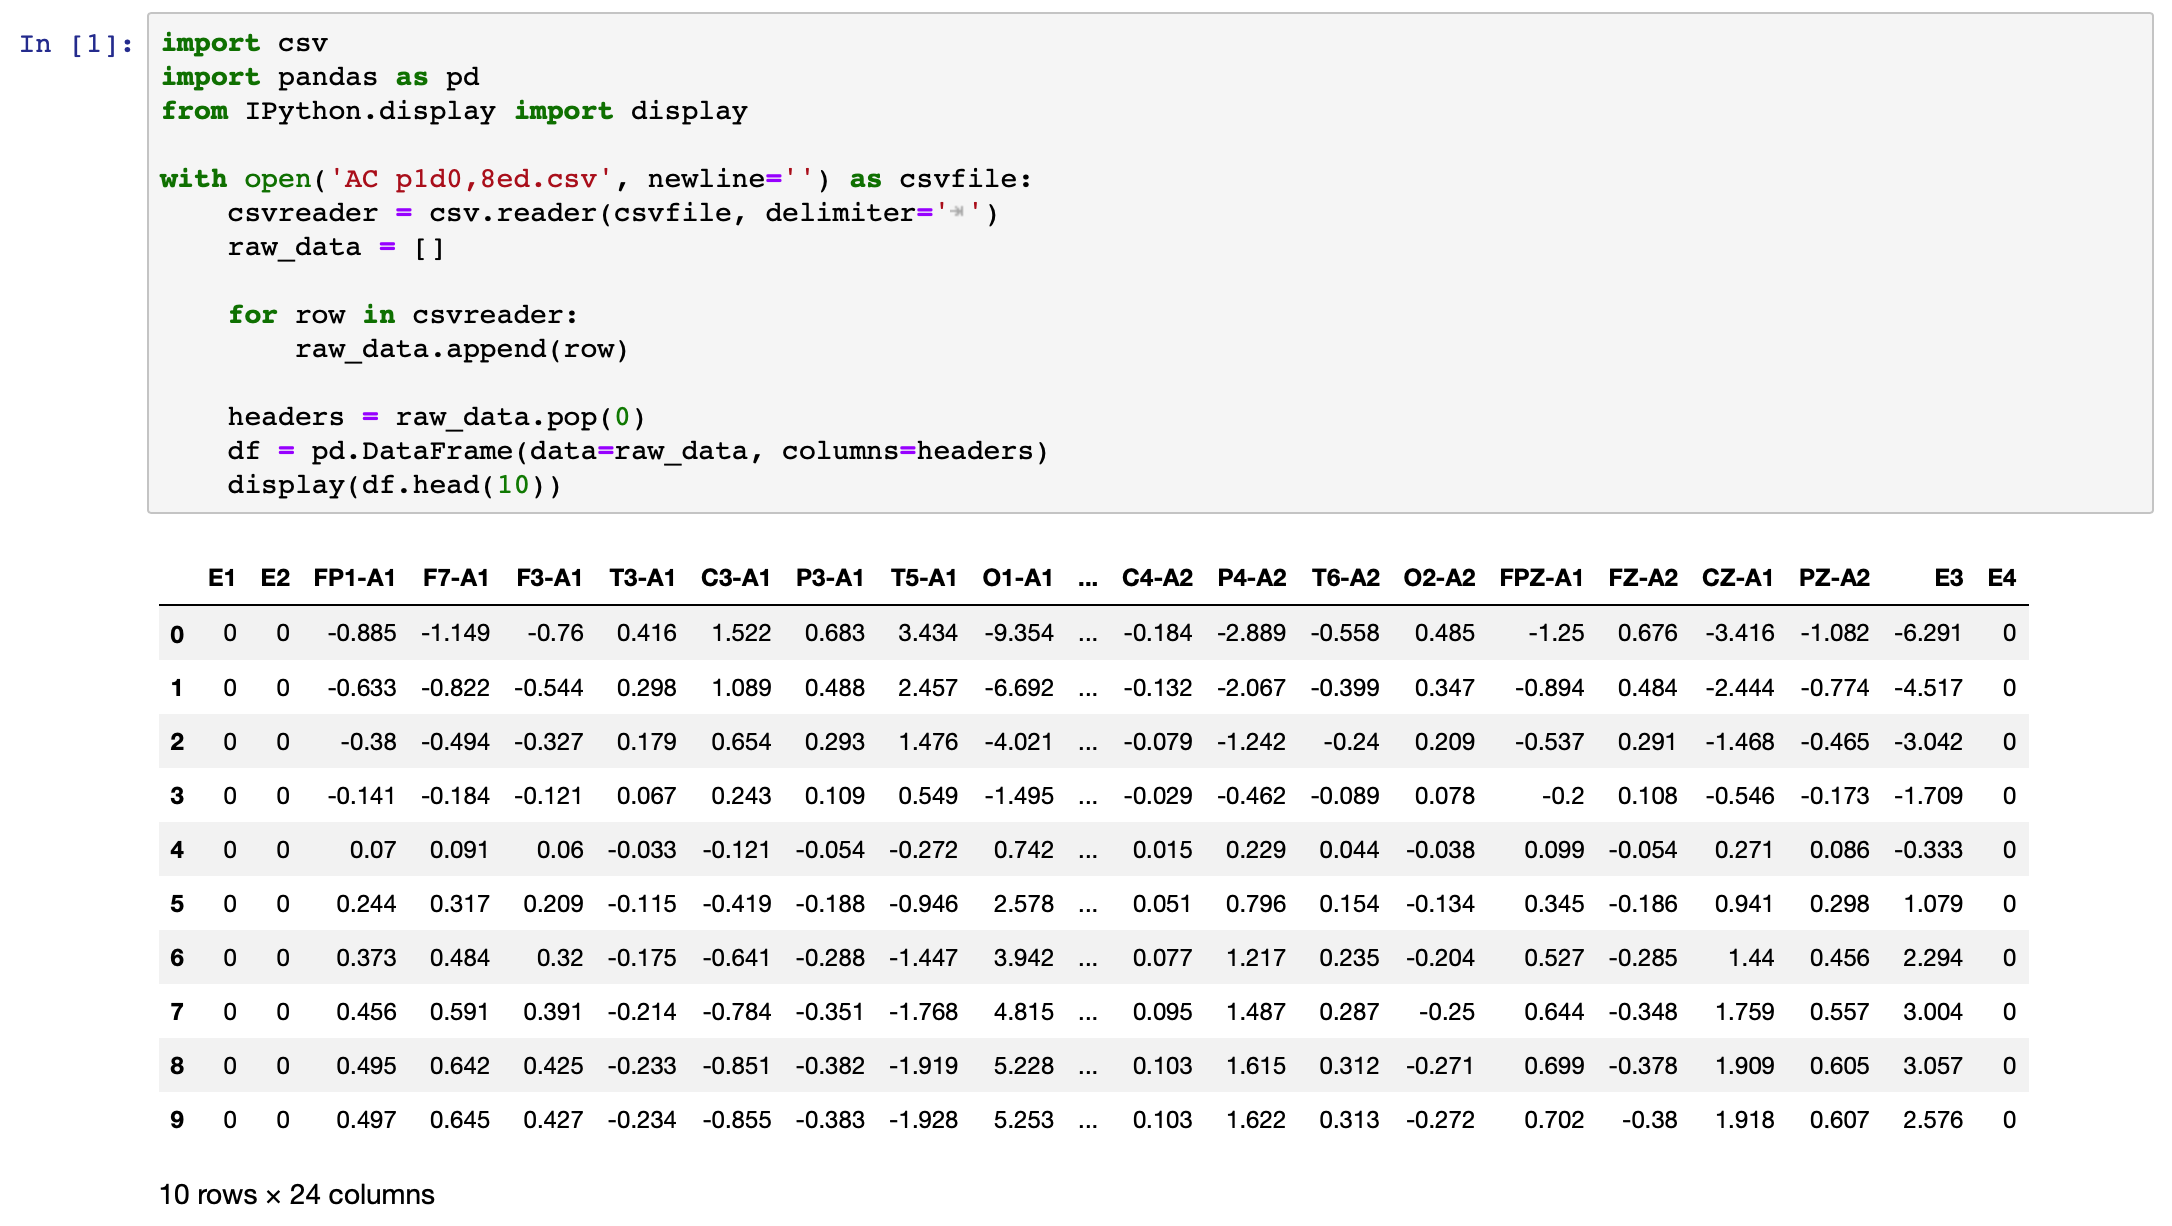
\includegraphics[scale=0.45]{1.png}
    \caption{Исходные данные}
\end{figure}

%%%%%%%%%%%%%%%%%%%%%%%%%%%%%%%%%%%%%%%%%%%%%%%%%%%
% % % % % % % % Глава 2 % % % % % % % % 
%%%%%%%%%%%%%%%%%%%%%%%%%%%%%%%%%%%%%%%%%%%%%%%%%%%

\chapter{Основное содержание работы}

\textbf{Во введении} обосновывается актуальность исследования, ставятся цели и задачи, определятся предмет и объект исследования, постулируются основные проблемы исследования и способы их решения, описывается научная новизна и практическая ценность работы.

\textbf{В первой главе} вкратце рассматривается история изучения эпилепсии как болезни, различные подходы к классификации данных и попытки предсказать приступы, которые предпринимались в прошлом.

\textbf{Вторая глава} посвящена анализу входных данных, поступающих с различных датчиков ЭЭГ, предварительной обработке и анализу этих данных, описанию используемых алгоритмов и демонстрации кода.

Входные данные с различных данных, представленные в виде списка:

\begin{figure}[h!]
    \centering
    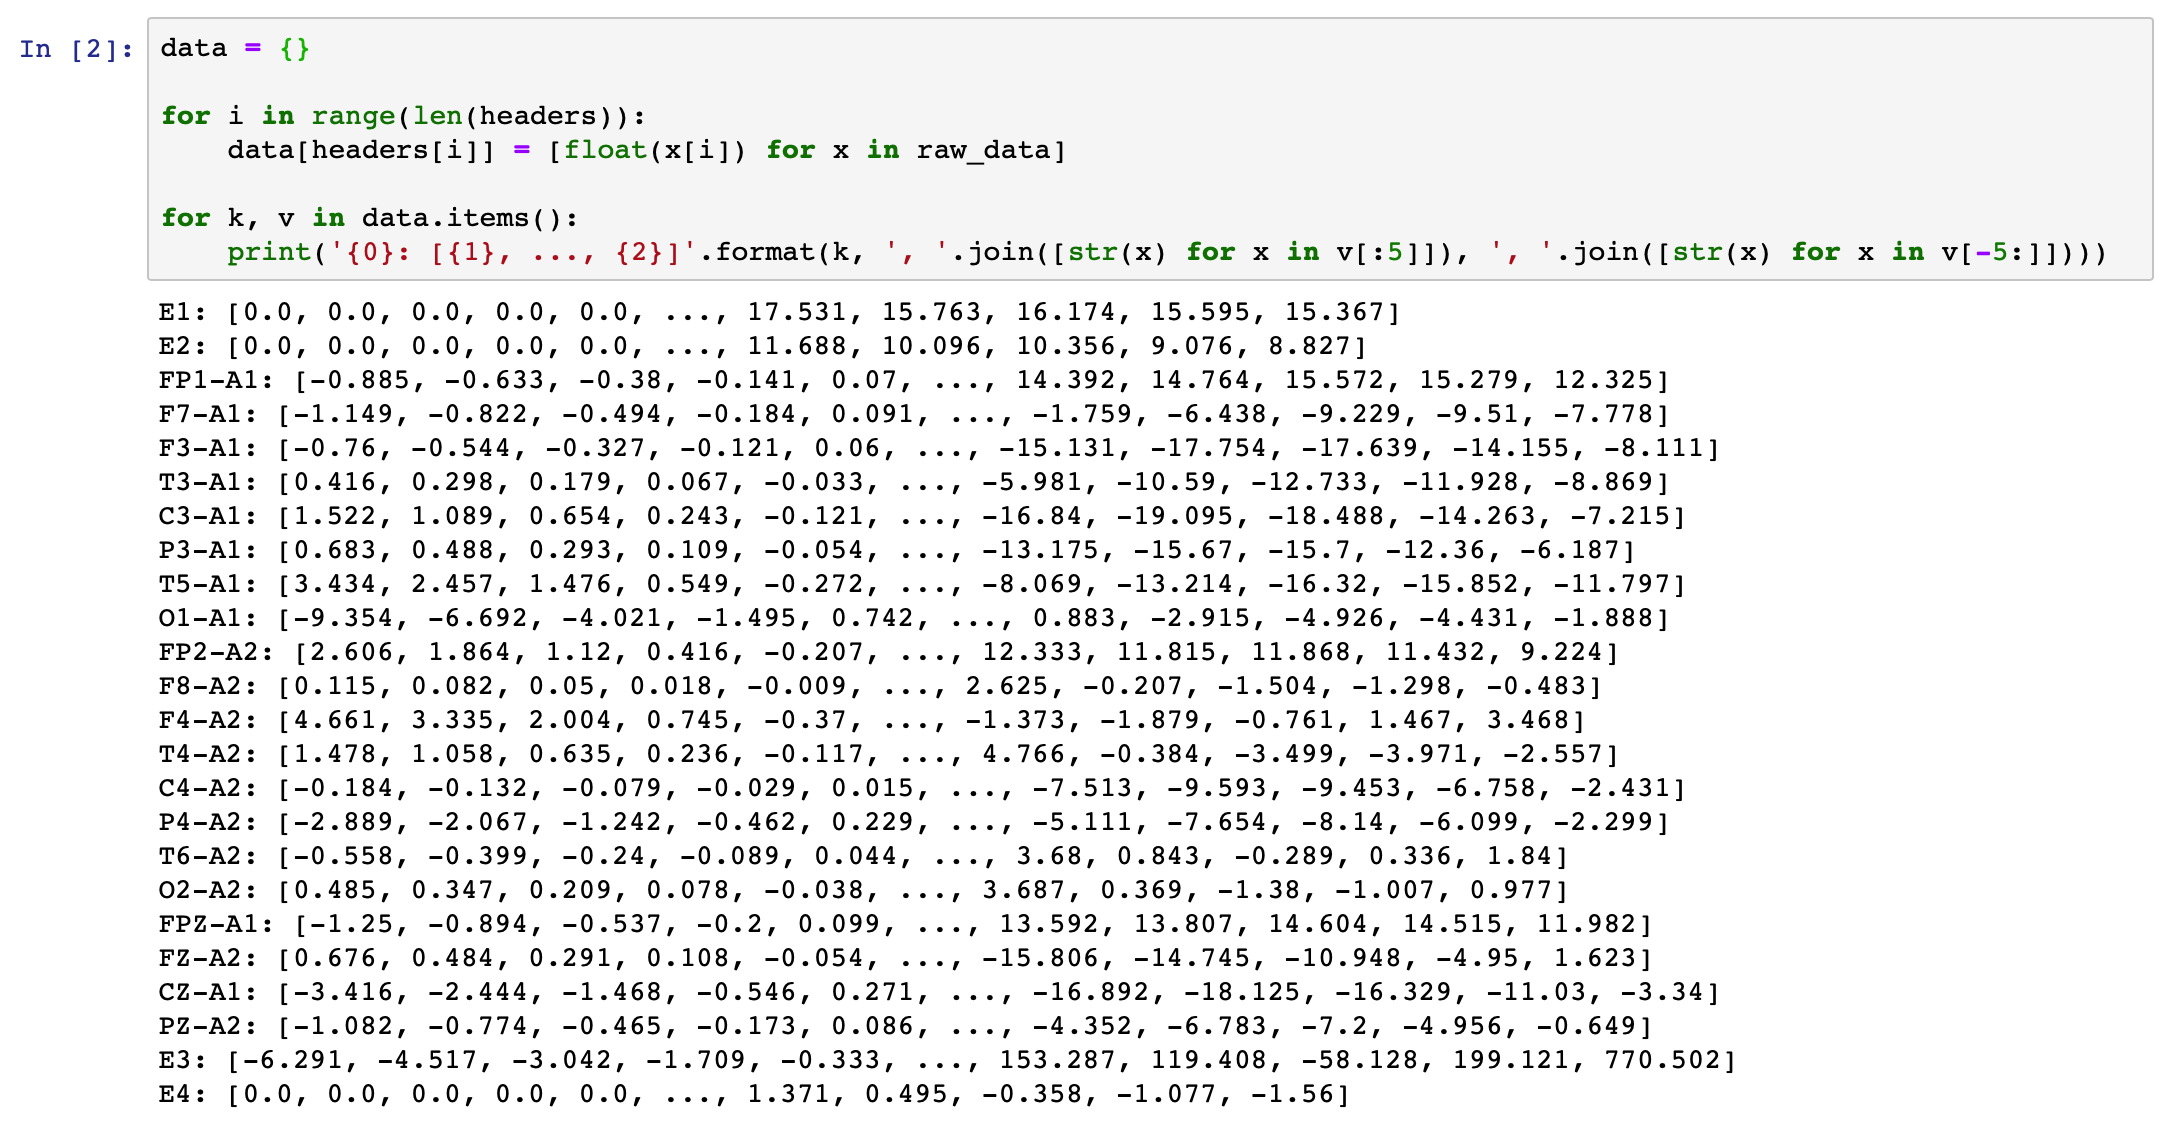
\includegraphics[scale=0.4]{2.png}
    \caption{Исходные данные в виде списков}
\end{figure}

\newpage
График показаний одного датчика (каждое 1000-е измерение):

\begin{figure}[h!]
    \centering
    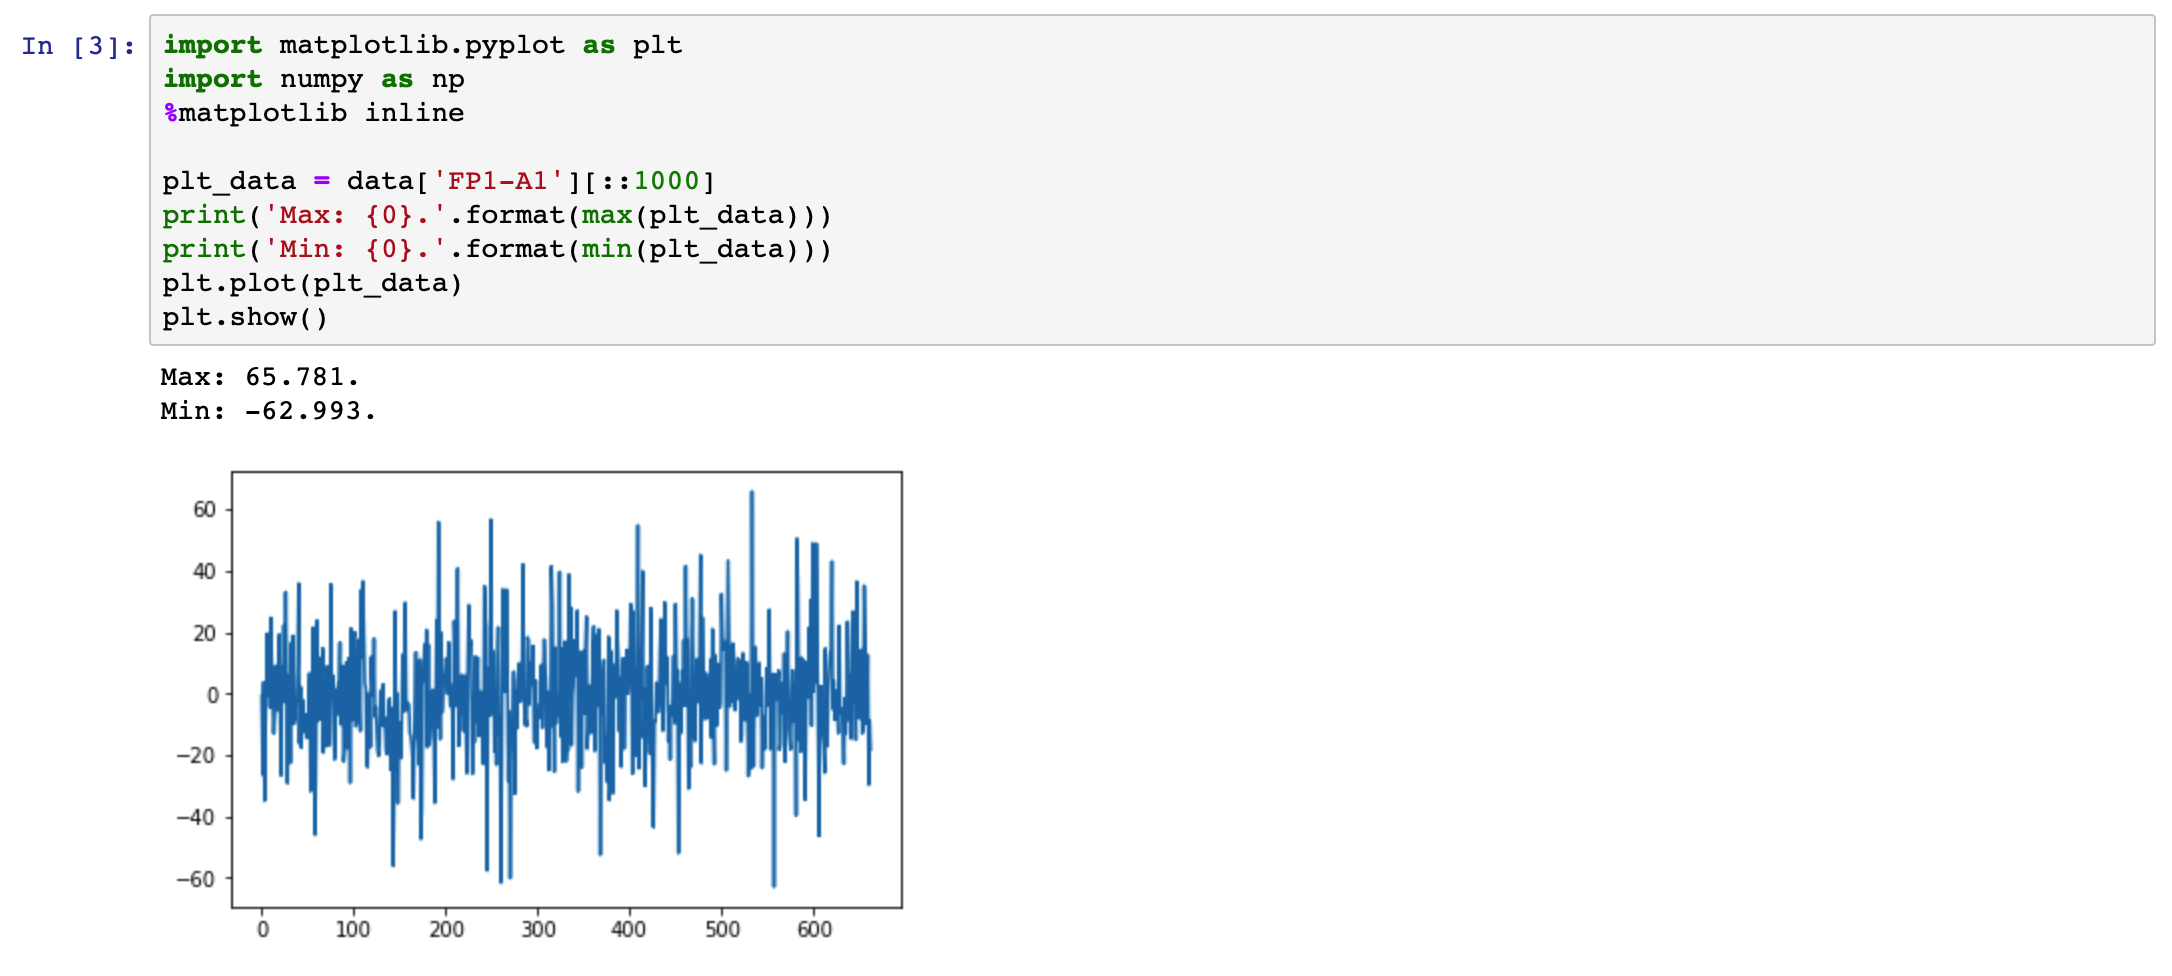
\includegraphics[scale=0.45]{3.png}
    \caption{Исходные данные в виде списков}
\end{figure}

\textbf{В третьей главе} проводится основная математическая и алгоритмическая работа над полученными данными. Производится построение динамической системы и строится предиктор эпилептического приступа.

\textbf{Четвёртая глава} посвящена теоретическим выкладкам, в которых производится попытка теоретически обосновать результаты работы каждого шага полученного алгоритма.

И, наконец, \textbf{в заключении} собираются воедино все полученные в данной работе результаты. Описывается алгоритм построения предиктора эпилептического приступа по данным электроэнцефалограмм. Формулируются основные теоретические выводы, полученные в работе, описывается возможное дальнейшее направление работы и способы применения полученных алгоритмов.

%%%%%%%%%%%%%%%%%%%%%%%%%%%%%%%%%%%%%%%%%%%%%%%%%%%
% % % % % % % % Глава 3 % % % % % % % % 
%%%%%%%%%%%%%%%%%%%%%%%%%%%%%%%%%%%%%%%%%%%%%%%%%%%

\chapter{Заключение}

В результате работы были получены следующие важные результаты:

\begin{enumerate}
    \item Были исследованы реальные данные, поступающие с датчиков электроэнцефалограмм реальных пациентов.
    \item Были исследованы временные ряды и соответствующие динамические системы, построена математическая модель.
    \item Был построен предиктор эпилептического приступа.
\end{enumerate}

%%%%%%%%%%%%%%%%%%%%%%%%%%%%%%%%%%%%%%%%%%%%%%%%%%%
% % % % % % % % Список литературы % % % % % % % % 
%%%%%%%%%%%%%%%%%%%%%%%%%%%%%%%%%%%%%%%%%%%%%%%%%%%

\begin{thebibliography}{9}
\addcontentsline{toc}{chapter}{\bibname}

\bibitem{Orlov-bib1}
Ивченко А.Ю., Козлова А.Б., Корсакова М.Б., Машеров Е.Л., Орлов Ю.Н., Руссков А.А. \textit{Анализ нестационарности ЭКоГ и построение предвестника разладки} \\
\textbf{Препринты ИПМ им. М.В. Келдыша.} 2017. № 49. 19 с.

\end{thebibliography}
\end{document}
